\documentclass[10pt,twocolumn,letterpaper]{article}

\usepackage[margin=0.75in]{geometry}
\usepackage[T1]{fontenc}
\usepackage[utf8]{inputenc}
\usepackage{amsmath,amssymb,amsfonts,amsthm}
\usepackage{booktabs}
\usepackage{tabularx}
\usepackage{graphicx}
\usepackage{xurl}
\usepackage{hyperref}
\usepackage{microtype}
\usepackage{enumitem}
\usepackage{cite}
\usepackage{listings}
\usepackage{color}
\usepackage{orcidlink}

\setlength{\textfloatsep}{14pt plus 3pt minus 2pt}
\setlength{\floatsep}{10pt plus 2pt minus 2pt}
\setlength{\intextsep}{10pt plus 2pt minus 2pt}
\setlength{\dbltextfloatsep}{14pt plus 3pt minus 2pt}
\setlength{\dblfloatsep}{10pt plus 2pt minus 2pt}
\setlength{\abovecaptionskip}{8pt plus 2pt minus 1pt}
\setlength{\belowcaptionskip}{8pt plus 2pt minus 1pt}

\hypersetup{
  colorlinks=true,
  linkcolor=blue,
  citecolor=blue,
  urlcolor=blue
}

\newtheorem{theorem}{Theorem}
\newtheorem{proposition}{Proposition}
\newtheorem{definition}{Definition}
\newtheorem{lemma}{Lemma}

\definecolor{codegreen}{rgb}{0,0.6,0}
\definecolor{codegray}{rgb}{0.5,0.5,0.5}
\definecolor{codepurple}{rgb}{0.58,0,0.82}
\definecolor{backcolour}{rgb}{0.97,0.97,0.97}

\lstdefinestyle{leanstyle}{
    backgroundcolor=\color{backcolour},   
    commentstyle=\color{codegreen},
    keywordstyle=\color{blue},
    numberstyle=\tiny\color{codegray},
    stringstyle=\color{codepurple},
    basicstyle=\ttfamily\fontsize{5.8pt}{7.0pt}\selectfont,
    breakatwhitespace=false,         
    breaklines=true,                 
    captionpos=b,                    
    keepspaces=true,                 
    numbers=left,                    
    numbersep=5pt,                  
    xleftmargin=18pt,
    framexleftmargin=18pt,
    showspaces=false,                
    showstringspaces=false,
    showtabs=false,                  
    tabsize=2
}
\lstset{style=leanstyle}

\title{\textbf{From Grokking to Micro-Routing: Graph Neural Cellular Automata for Sub-Millisecond Agent Tool Selection}}
\author{%
  \textbf{Julian M. Kleber}\,\orcidlink{0000-0001-5518-0932} \\
  \textit{Independent Researcher} \\
  \texttt{julian.m.kleber@gmail.com}
}
\date{October 2026}

\begin{document}
\maketitle

\begin{abstract}
Selecting which tool to invoke in an autonomous software agent is fundamentally a micro-routing decision, yet current architectures dispatch every turn through multi-billion-parameter LLMs. We introduce \textbf{Graph Neural Cellular Automata (GNCA)}, an ultra-lightweight ($35.3\text{k}$--$59.2\text{k}$ parameter) System-1 reflex router that selects tools via recurrent message passing on a relational trace graph. Using \textbf{Lean 4}, we machine-check structural invariants of candidate discrete topologies prior to training (1D lattice subsumption, tree subsumption, star-vs-chain diameter separation $O(1)$ vs $\Omega(V)$, and permutation equivariance) with zero unproven axioms. We further verify empirically that top-$k=2$ discretization of trained meta-learned adjacency matrices recovers the verified call-tree subgraph with goal eccentricity $2$. GNCA delivers \textbf{sub-millisecond routing latency}, executing batch-1 forward passes in $\mathbf{0.35}$--$\mathbf{0.66\text{ ms}}$ on CPU ($18\ \mu\text{s}$ on GPU) compared to $42.1\text{ ms}$ for local small LLMs. On the curated Hermes benchmark (3{,}530 test turns), 10k-step class-weighted GNCA variants reach $64.64\%$--$66.19\%$ test top-1. This trails converged tabular baselines (Random Forest $67.88\%$ test, HistGradientBoosting $69.47\%$ test) on top-1 while leading on test macro-F1 ($0.584$--$0.608$ vs $0.283$ Random Forest). Under unweighted label-smoothed cross-entropy ($K=8$, $59.2\text{k}$ parameters), GNCA reaches $67.37\%$ test top-1 at the matched 10k-step snapshot. Across a 200k-step grokking horizon, it reaches $\mathbf{68.07\%}$ test top-1 ($[66.49, 69.60]\%$), matching Random Forest ($\Delta = +0.19\text{ pp}$, paired $p=0.72$). Multi-seed evaluation on BFCL v4 ($N=692$ test turns) confirms cross-corpus generalization ($\mathbf{75.24\%}$ test top-1 vs $74.47\%$ Random Forest, paired $p=0.35$) and significant gains over random routing in matched-actuator ablations.
\end{abstract}

\section{Introduction}
Autonomous software agents operate as iterative closed-loop systems: observing environment feedback (compiler diagnostics, file diffs, test logs) and synthesizing next actions. In biological nervous systems, routine motor actions do not require deliberative processing in the cerebral cortex; a low-level reflex arc in the spinal cord coordinates rapid responses in milliseconds. In contrast, modern AI agents dispatch every mundane operation through massive, multi-billion-parameter autoregressive models. This design causes critical bottlenecks:
\begin{enumerate}[leftmargin=1.5em, itemsep=0.1em]
  \item \textbf{Latency and Memory Pressure.} Generating tokens sequentially causes high latency and heavy memory traffic, slowing down agent loops.
  \item \textbf{Context Window Bloat.} Intermediate steps fill context windows with repetitive JSON schema and syntax clutter.
  \item \textbf{Rigid 1D Assumptions.} Prior cellular models restrict computation to 1D lattices. Signals crawl one step at a time like a game of telephone, ignoring that agent execution traces form hierarchical trees.
\end{enumerate}

Neural Cellular Automata (NCAs)~\cite{mordvintsev2020growing} offer an alternative computational paradigm based on local, self-organizing update rules. Historically, NCAs were studied in continuous 2D grids for biological morphogenesis, texture generation, and self-repair. However, their core inductive biases (iterative spatial message passing across discrete cells governed by uniform update rules) align naturally with structured sequential decision processes. Like biological cells communicating with their immediate neighbors to form complex tissues, NCA cells update their local states in parallel without global bottlenecking. Recent investigations (e.g., Mittal et al.~\cite{mittal2026textnca}) probed token-level text NCAs, but their application to structured multi-action tool execution has remained limited to rigid sequential chains.

\paragraph{Contributions.} In this paper, I extend Neural Cellular Automata beyond 1D topologies into a graph framework for hierarchical agent routing (fixed star/tree baselines plus optional continuous architecture search). My core contributions are fourfold:
\begin{itemize}[leftmargin=1.5em, itemsep=0.1em]
  \item \textbf{Graph Cellular Automata:} I formulate GNCA, replacing 1D convolutional stencils with learned graph message passing. On curated Hermes test traces ($N=3{,}530$), 10k-step class-weighted variants reach $65.33\%$ test top-1 for meta-learned topology and $66.19\%$ test top-1 for star topology ($K{=}4$). Under unweighted label smoothing ($K{=}8$), Deep Tree GNCA reaches $67.37\%$ test top-1 at 10k steps and $68.07\%$ test top-1 across a 200k-step grokking trajectory, with cross-corpus transfer on BFCL v4 ($75.24\%$ test top-1).
  \item \textbf{Machine-Checked Structural Invariants \& Empirical Bridge:} In Lean 4, I formally verify 1D lattice subsumption, tree subsumption, and permutation equivariance with zero unproven axioms, and prove an exponential diameter gap between idealized star and chain topologies ($O(1)$ vs $\Omega(V)$). To bridge these discrete proofs to the deployed continuous softmax relaxation, I audit the archived $\alpha$ matrices across all random seeds. Hard top-$k=2$ row discretization recovers the verified binary call-tree subgraph with goal eccentricity $2$.
  \item \textbf{Dual-System Architecture:} I introduce a high-throughput System-1/System-2 agent harness with risk-gated dynamic schema pruning, filtering non-candidate tools before LLM actuation and validating the normalized step-norm escalation score empirically across $3{,}530$ held-out test turns.
  \item \textbf{Controlled Router Ablations \& Exploratory Pilot Diagnostics:} Using matched-actuator router ablations on $N=692$ BFCL v4 test turns, I isolate the router's contribution over random and no-router baselines while holding the harness fixed. I complement this with exploratory end-to-end pilot diagnostics ($N=10$ $\tau^2$-bench tasks, $N=30$ BFCL probes, one SWE episode; \texttt{EXP-20261102-003}).
\end{itemize}

\section{Related Work}

\paragraph{Neural Cellular Automata and Reasoning.}
Mordvintsev et al.~\cite{mordvintsev2020growing} introduced Growing Neural Cellular Automata, demonstrating self-organizing pattern morphogenesis and damage recovery. Subsequent work extended NCAs to multi-scale hierarchical structures~\cite{pande2023hierarchical} and decentralized algorithmic reasoning~\cite{etcheverry2026reasoning}. Grattarola et al.~\cite{grattarola2021learning} introduced Learning Graph Cellular Automata (LGCA), showing that GNNs can execute cellular update rules over fixed, predefined graphs (e.g., Voronoi meshes). In language representation, Mittal et al.~\cite{mittal2026textnca} and Lee et al.~\cite{lee2026training} demonstrated that cellular rules can learn 1D token representations. My framework departs from token generation and static GCA. Because agent traces lack a predefined graph, I introduce hand-crafted broadcast topologies and continuous architecture search. I combine these with cross-turn carry and Lean 4 proofs of structural invariants.

\paragraph{Tool Calling, Agent Harnesses, and Pre-Routing.}
Tool use in autonomous systems is evaluated on benchmarks like the Berkeley Function Calling Leaderboard (BFCL)~\cite{gorilla-bfcl} and SWE-bench. Production agent harnesses execute many typed System-1 decisions per task~\cite{li2026fastmodels}. Singla et al.~\cite{singla2026agentweave} showed that pre-inference action routing cuts prompt latency and token overhead by half. Expanding on these findings, real agents must handle three coupled tasks: detecting irrelevance to abstain gracefully, binding argument slots to workspace entities, and coordinating multi-turn plans.

\paragraph{Architecture Meta-Learning \& Graph Bottlenecks.}
Standard GNNs frequently suffer from \emph{oversmoothing} (representations collapsing to uniformity with depth), \emph{oversquashing} (information bottlenecking from high-degree neighborhoods), and \emph{underreaching} (insufficient message passing depth to bridge distant nodes). By casting topology selection as bilevel architecture meta-learning (optional) or fixed star/tree wiring, the framework targets sparse relational graphs that balance local message passing with long-range goal broadcasting.

\section{Task Formulation \& Architecture}

\subsection{Real-World Operational Context \& Action Formulation}
In real-world software engineering agents (e.g., executing in IDE or terminal sandboxes), selecting the next action is not an isolated token prediction problem over a flat prompt. Instead, the agent operates in an interactive closed loop situated within an operational context state $\mathbf{s}_t$.
\begin{equation}
  \mathbf{s}_t = \left(\mathbf{g}_{\text{intent}}, \; \mathbf{w}_{\text{env}}, \; \mathbf{\tau}_{\text{hist}}, \; \mathcal{T}_{\text{reg}}\right) \in \mathcal{X}_{\text{ctx}}
\end{equation}
The four context channels capture the heterogeneous dependencies of practical workflows:
\begin{enumerate}[leftmargin=1.5em, itemsep=0.1em]
  \item \textbf{High-Level Intent ($\mathbf{g}_{\text{intent}}$):} The user goal, issue specification, or immediate task turn defining the overarching objective.
  \item \textbf{Workspace \& Environment State ($\mathbf{w}_{\text{env}}$):} File paths, working directory depth, git branch/clean status, compiler and test exit codes, and runtime error diagnostics.
  \item \textbf{Causal Trajectory History ($\mathbf{\tau}_{\text{hist}}$):} Chronological sequence of prior tool calls and execution feedback $\mathbf{\tau}_{\text{hist}} = \{(u_{t-k}, r_{t-k})\}_{k=1}^{L-1}$ over an $L$-step causal window. Here $u_{t-k} \in \mathcal{V}$ is the invoked tool and $r_{t-k}$ contains execution diagnostics (output length, error flag, stdout/stderr status).
  \item \textbf{Tool Registry \& Schema Constraints ($\mathcal{T}_{\text{reg}}$):} Candidate tool signatures $|\mathcal{V}|$, argument constraints, and permission boundaries (read-only introspection vs state-mutating shell execution).
\end{enumerate}

From this context $\mathbf{s}_t$, the agent synthesizes a four-part action tuple:
\begin{equation}
  \mathbf{a}_t = \left(y_{\text{tool}}, \; \mathbf{y}_{\text{arg}}, \; g_{\text{abstain}}, \; \tau_{\text{escalate}}\right)
\end{equation}
Here $y_{\text{tool}} \in \mathcal{V}$ is the discrete tool identifier chosen from vocabulary $|\mathcal{V}| = 13$ (e.g., \texttt{read\_file}, \texttt{edit\_file}, \texttt{run\_command}, \texttt{list\_dir}, \texttt{respond}). The vector $\mathbf{y}_{\text{arg}} \in \mathcal{A}$ predicts structured argument slots mapping workspace entities. The calibrated scalar gate $g_{\text{abstain}} \in [0, 1]$ indicates whether the agent should abstain from external tool execution. Finally, $\tau_{\text{escalate}} \in [0, 1]$ provides a predictive execution risk score governing System-2 LLM fallback.

\subsection{Beyond 1D: Graph Neural Cellular Automata}
Standard 1D NCAs constrain message passing strictly to immediate sequence neighbors $\{i-1, i, i+1\}$, forcing contextual signals to crawl sequentially across $\Omega(V)$ steps. In agent workflows, however, the root goal and environmental diagnostics must directly modulate every historical turn, while recursive tool subtrees branch hierarchically.

I map the operational context $\mathbf{s}_t$ to an expressive relational graph $\mathcal{G} = (\mathcal{V}_{\text{graph}}, \mathcal{E}, A)$ with $|\mathcal{V}_{\text{graph}}| = V = 5$ nodes over a causal window $L=5$.
\begin{itemize}[leftmargin=1.5em, itemsep=0.1em]
  \item \textbf{Node $0$ (Intent \& Environment Hub):} Anchors the global intent $\mathbf{g}_{\text{intent}}$ concatenated with workspace diagnostic scalars $\mathbf{w}_{\text{env}}$.
  \item \textbf{Nodes $1 \dots 4$ (Causal Trajectory Cells):} Chronological execution turns $(u_{t-k}, r_{t-k})$, capturing both the historical operation and runtime feedback.
\end{itemize}
Each node maintains a compact 16-number scratchpad ($h_i^{(t)} \in \mathbb{R}^{16}$, initialized to $\mathbf{0}$). Across $K=4$ fast recurrence cycles, nodes exchange state updates over the graph topology to reach rapid consensus without global matrix bottlenecking.

\paragraph{Continuous Spatial Perception.}
Let $A \in \mathbb{R}^{V \times V}$ denote a \textbf{row-stochastic} adjacency ($A_{ij} \ge 0$, $\sum_{j=1}^V A_{ij} = 1$ for all $i$). Adjacency $A$ can be fixed or continuously parameterized via row-wise $\mathrm{softmax}(\alpha/\tau)$. Each cell carries a concatenated observation--hidden vector $x_i^{(t)} \in \mathbb{R}^{C}$ with $C = D + H$, where hidden width $H{=}16$. Stacking $x_i^{(t)}$ yields observation matrix $x^{(t)} \in \mathbb{R}^{V \times C}$. Neighbor aggregation is a left multiply by $A$ for low-pass consensus.
\begin{equation}\label{eq:gnca-lowpass}
  \bar{x}_i^{(t)} = \sum_{j=1}^V A_{ij}\, x_j^{(t)} \quad \Leftrightarrow \quad \bar{\mathbf{x}}^{(t)} = A\,\mathbf{x}^{(t)}.
\end{equation}
The high-pass channel computes the directed difference operator $(A - I)\mathbf{x} = -(I - A)\mathbf{x}$ on the same row-stochastic adjacency $A$.
\begin{equation}\label{eq:gnca-highpass}
  \delta_i^{(t)} = \sum_{j=1}^V A_{ij}\bigl(x_j^{(t)} - x_i^{(t)}\bigr) \quad \Leftrightarrow \quad \boldsymbol{\delta}^{(t)} = (A - I)\,\mathbf{x}^{(t)}.
\end{equation}
In directed graph signal processing, $L_{\text{rw}} = I - A$ is the standard random-walk graph Laplacian for asymmetric causal routing graphs. Its row sums vanish ($\sum_j (A_{ij} - \delta_{ij}) = 0$), so $(A - I)\mathbf{x}$ vanishes on spatially constant states. It thus isolates the directed local gradient $\bar{x}_i^{(t)} - x_i^{(t)}$ away from neighborhood consensus without requiring symmetric degree normalization.
The perception tensor stacks identity, low-pass, and high-pass channels along the feature axis. This construction mirrors classical NCAs~\cite{mordvintsev2020growing} on the trace graph.
\begin{equation}\label{eq:gnca-perceive}
  p_i^{(t)} = \left[ x_i^{(t)}, \; \bar{x}_i^{(t)}, \; \delta_i^{(t)} \right] \in \mathbb{R}^{3C}.
\end{equation}

\paragraph{Pointwise State Update.}
A shared 1$\times$1 convolution over the $3C$-channel perceived tensor computes the gated state update $\Delta h_i^{(t)} \in \mathbb{R}^{H}$ from $p_i^{(t)}$.
\begin{equation}
  [\tilde{\Delta} h_i^{(t)}, \; g_i^{(t)}] = W_2 \, \operatorname{ReLU}(W_1 p_i^{(t)} + b_1), \quad \Delta h_i^{(t)} = \sigma(g_i^{(t)}) \odot \tilde{\Delta} h_i^{(t)}
\end{equation}
Here $W_1 \in \mathbb{R}^{D_{\mathrm{mid}} \times 3C}$, $b_1 \in \mathbb{R}^{D_{\mathrm{mid}}}$, $W_2 \in \mathbb{R}^{2H \times D_{\mathrm{mid}}}$, and $D_{\mathrm{mid}} = 96$. Per-cell observation width is $D = d_{\text{svd}} + 4 + |\mathcal{V}| + 1$. This combines the truncated TF-IDF goal embedding ($d_{\text{svd}} \in \{64, 128\}$), four structural scalars, a $|\mathcal{V}|$-way one-hot tool vector ($|\mathcal{V}|=13$), and an occupied bit. As derived in Appendix~\ref{sec:appendix-params} (Table~\ref{tab:param-derivation}), the cellular update and readout sum to $288D + 17{,}134$ trainable parameters for fixed topologies ($+25$ for meta-learned $\alpha \in \mathbb{R}^{5 \times 5}$, and $+64$ for $K=8$ step embeddings). Thus $D=146$ (SVD128 in \texttt{EXP-20261102-001}) yields $59{,}182$ parameters for fixed topologies, $59{,}207$ for meta-learned topology, and $59{,}246$ for $K=8$ Deep Tree (\texttt{EXP-20261102-002}). The compact $D=82$ (SVD64) configuration yields $35{,}347$ ($35.3\text{k}$) parameters.

\paragraph{Residual State Accumulation.}
Updates are applied residually across $K=4$ cycles:
\begin{equation}
  h_i^{(t+1)} = h_i^{(t)} + m_i^{(t)} \odot \Delta h_i^{(t)}
\end{equation}
where $m_i^{(t)} \sim \operatorname{Bernoulli}(p)$ ($p=0.8$ during training; $1.0$ at inference) enforces asynchronous cellular computation.

\subsection{Architecture Meta-Learning on Spatial Topologies}
To reduce manual topology tuning, I also formulate an optional bilevel architecture meta-learning problem.
\begin{equation}
  \begin{aligned}
    \min_{\alpha \in \mathbb{R}^{V \times V}} \; & \mathcal{L}_{\text{val}}\left(\theta^*(\alpha); \; A^{(\alpha)}\right) \\
    \text{s.t.} \; & \theta^*(\alpha) = \arg\min_\theta \mathcal{L}_{\text{train}}(\theta; \; A^{(\alpha)})
  \end{aligned}
\end{equation}
The continuous matrix $\alpha \in \mathbb{R}^{V \times V}$ parameterizes edge probabilities via a row-wise softmax relaxation across candidate source nodes.
\begin{equation}
  A_{ij}^{(\alpha)} = \frac{\exp(\alpha_{ij} / \tau)}{\sum_{k=1}^V \exp(\alpha_{ik} / \tau)}
\end{equation}
The bilevel architecture optimization problem is solved using a first-order DARTS gradient approximation on $\mathcal{L}_{\text{val}}$, annealing softmax temperature $\tau$ from $1.0 \to 0.1$. \textbf{Primary benchmark runs} (\texttt{EXP-20261102-001}) keep a \textbf{continuous} row-softmax adjacency $A^{(\alpha)}_{ij} = \mathrm{softmax}_j(\alpha_{ij}/\tau)$ during training and evaluation. To connect the continuous softmax adjacency to the discrete Lean-verified graph families, we evaluate hard top-$k=2$ row discretization ($A_{\text{disc}}^{(k=2)}$, retaining the $k=2$ largest weights per row) on all archived meta-learned checkpoints in Section~\ref{sec:formal-verification}. Fixed baselines interpolate between 1D chains ($A_{\text{1D}}$), star goal-broadcasting ($A_{\text{star}}$), and hierarchical call trees ($A_{\text{tree}}$).

\subsection{Hierarchical Multi-Head Readout \& Dual-System Escalation}\label{sec:dual-system}
After $K$ iterations, the spatial grid $\mathbf{H}^{(K)} \in \mathbb{R}^{V \times H}$ is decoded via four specialized readout heads.
\begin{enumerate}[leftmargin=1.5em, itemsep=0.1em]
  \item \textbf{Tool Classification Head:} The spatial grid projects to tool logits.
  \begin{equation}
    \hat{y}_{\text{tool}} = \operatorname{softmax}\left(W_{\text{tool}} \operatorname{vec}(\mathbf{H}^{(K)}) + b_{\text{tool}}\right)
  \end{equation}
  \item \textbf{Argument Slot Head:} Bilinear interactions between goal and history cells are computed.
  \begin{equation}
    \hat{\mathbf{y}}_{\text{arg}} = \operatorname{softmax}\left({h_0^{(K)}}^\top W_{\text{arg}} h_{\text{last}}^{(K)}\right)
  \end{equation}
  \item \textbf{Abstain Gate:} A scalar gate flags irrelevant contexts.
  \begin{equation}
    g_{\text{abstain}} = \sigma\left(w_{\text{abs}}^\top h_0^{(K)} + b_{\text{abs}}\right)
  \end{equation}
  \item \textbf{Uncertainty Score:} Prediction entropy and final-step state delta magnitude are combined into a \textbf{unitless} heuristic risk score calibrated on the validation split and empirically validated on held-out turns.
  \begin{equation}\label{eq:escalate}
    \tau_{\text{escalate}} = \underbrace{\frac{\mathcal{H}(\hat{y}_{\text{tool}})}{\log |\mathcal{V}|}}_{\in [0,1]} + \beta \underbrace{\frac{1}{V \sqrt{H}} \sum_{i=1}^V \|\Delta h_i^{(K-1)}\|_2}_{\text{mean normalized } \ell_2 \text{ step norm}}
  \end{equation}
  Both summands are dimensionless: tool entropy is normalized by $\log |\mathcal{V}| \in [0, 1]$, and under isotropic hidden updates with per-channel variance $\sigma^2$, the Euclidean norm scales as $\mathbb{E}[\|\Delta h_i\|_2] \approx \sigma \sqrt{H}$. Dividing by $V\sqrt{H}$ ($1/(5\sqrt{16}) = 0.05$) yields a graph-size- and width-invariant $\mathcal{O}(1)$ quantity. \textbf{Empirical distribution validation:} Across all $3{,}530$ held-out turns of the curated Hermes test split (\texttt{stage0/stage0\_results/step\_norm\_distribution\_audit.json}), the normalized step-norm term at the best-validation checkpoint (\texttt{best\_graph\_nca\_grokking.pt}) has empirical mean $0.420 \pm 0.091$ (median $0.405$, 5th--95th percentile $[0.300, 0.590]$). At the 10k-step checkpoint (\texttt{graph\_nca\_step\_010000.pt}), it has mean $0.482 \pm 0.113$ (median $0.463$, 5th--95th percentile $[0.340, 0.687]$). This matches the empirical scale of the normalized entropy term on the same split (mean $0.345 \pm 0.154$, median $0.348$, 5th--95th percentile $[0.097, 0.606]$). Under equal weighting ($\beta=1.0$) or balanced weighting ($\beta=0.5$) calibrated on validation, the combined score has empirical mean $0.765 \pm 0.153$ (median $0.768$, 5th--95th percentile $[0.523, 1.014]$). This calibrates $\tau_{\text{escalate}} = 0.76$ to the held-out median uncertainty boundary ($51.7\%$ escalation rate). Crucially, $\beta$ and $\tau_{\text{escalate}}$ govern Dual-System escalation and schema pruning only; they do \emph{not} affect standalone tool top-1 in Tables~\ref{tab:primary}--\ref{tab:feature-eval}.
\end{enumerate}

\section{Structural Properties \& Formal Verification}\label{sec:formal-verification}
To provide sound structural foundations, I formally verify four core structural invariants governing the candidate discrete topology space and conditional dynamical stability of the Graph NCA architecture class. Machine-checked statements (formal Lean theorems) include:
\begin{itemize}[leftmargin=1.5em, itemsep=0.05em]
  \item \texttt{theorem\_subsumption\_1d}: the 1D lattice adjacency \texttt{lineGraphAdj} is realizable in the search space.
  \item \texttt{star\_graph\_diameter\_two}: every pair in \texttt{starSimpleGraph} is connected by a path of length $\le 2$.
  \item \texttt{line\_graph\_distance\_bound}: paths on the line graph advance node indices by at most one hop per step (yielding $\Omega(V)$ goal-to-tail separation).
  \item \texttt{theorem\_tree\_subsumption}: hierarchical tree adjacency \texttt{treeGraphAdj} is realizable.
  \item \texttt{neighborhood\_equivariance} / \texttt{path\_equivariance}: graph neighborhoods and paths commute with node permutations.
  \item \texttt{fixed\_point\_unique} / \texttt{trajectory\_decay}: conditional contraction implies unique fixed points and $2^{-n}$ perturbation decay.
\end{itemize}
All proofs compile in \textbf{Lean 4.35} with zero axioms. Theorem~\ref{thm:contraction} does \emph{not} assert that empirical SGD weights are contractive.

\begin{theorem}[Topological Subsumption]\label{thm:subsumption}
Let $\mathcal{T}_{\mathrm{1D}}$ denote the 1D circular or boundary-padded regular cellular automaton lattice on $V$ nodes. Then $\mathcal{T}_{\mathrm{1D}}$ is a strict element of the Graph Neural Cellular Automata topology space $\mathcal{S}_{\mathrm{GNCA}}$ under tridiagonal adjacency $A_{ij} = \mathbb{I}(|i - j| \le 1)$.
\end{theorem}

\begin{theorem}[Receptive Field Diameter Separation (idealized star vs.\ 1D chain)]\label{thm:diameter}
Fix $V \ge 3$. For the 1D nearest-neighbor lattice $\mathcal{G}_{\mathrm{1D}}$ in Lean (\texttt{lineSimpleGraph}), any directed path from goal node $0$ to terminal node $V{-}1$ has length at least $V{-}1 = \Omega(V)$ cellular hops. For the idealized \textbf{goal-broadcast star} $\mathcal{G}_{\mathrm{star}}$ (\texttt{starSimpleGraph} with hub at node $0$), every ordered pair $(u,v)$ is connected by a directed path of length at most $2$ (\texttt{star\_graph\_diameter\_two}). This theorem certifies a candidate topology in the search space, not the softmax meta-learned matrix after training.
\end{theorem}

\noindent\textbf{Empirical bridge between Lean-verified discrete topologies and trained continuous $\alpha$ weights.} Under the row-stochastic convention in Eqs.~\eqref{eq:gnca-lowpass}--\eqref{eq:gnca-highpass} ($j \to i$ when $A_{ij}>0$), fixed discrete topologies on $V{=}5$ trace nodes have directed diameters $4$ (1D), $2$ (star), and $3$ (tree). Their goal eccentricities from node $0$ are $4$, $1$, and $2$ respectively (\texttt{stage0/stage0\_results/topology\_diameter\_audit.json}). To connect deployed continuous row-softmax matrices $A^{(\alpha)} = \mathrm{softmax}(\alpha/\tau)$ to these discrete topologies, we audit all six archived meta-learned checkpoints in \texttt{stage0/stage0\_results/e3\_meta\_adjacency\_audit.json}.
\begin{enumerate}[leftmargin=1.5em, itemsep=0.05em]
  \item \textbf{Continuous Softmax Adjacency ($A^{(\alpha)}$).} Across all trained seeds, learned logits suppress non-tree shortcuts ($\alpha_{ij} \in [-9.17, -4.01]$, softmax weight $A_{ij}^{(\alpha)} \in [0.0001, 0.0068]$). Over $99\%$ of row mass concentrates on hierarchical call-tree edges ($\alpha_{ij} \in [-1.44, -0.01]$). Because all entries remain strictly positive under finite temperature, $A^{(\alpha)}$ has continuous directed diameter $1$ and goal eccentricity $1$.
  \item \textbf{Discretized Top-$k$ Adjacency ($A_{\text{disc}}^{(k=2)}$ and $A_{\text{disc}}^{(k=3)}$).} Applying hard top-$k=2$ row discretization to the trained $\alpha$ matrices recovers an exact subgraph of the Lean-verified binary call tree (\texttt{treeGraphAdj}, Theorem~\ref{thm:tree-subsumption}) across all six seeds. Root row $0$ retains $\{0, 1\}$ or $\{0, 2\}$ ($\approx [0.50, 0.50]$), while rows $1, 2$ retain $\{0, 1\}$ and $\{0, 2\}$. Leaf rows $3, 4$ retain $\{1, 3\}$ and $\{1, 4\}$ ($\approx [0.53, 0.47]$). Across all six trained checkpoints, $A_{\text{disc}}^{(k=2)}$ achieves directed goal eccentricity $\mathbf{2}$ from node $0$ and undirected tree diameter $\mathbf{3}$. Top-$k=3$ discretization retains all bidirectional parent--child edges with directed diameter $\mathbf{3}$ and goal eccentricity $\mathbf{2}$.
\end{enumerate}

\begin{theorem}[Neighborhood Permutation Equivariance]\label{thm:equivariance}
Let $\sigma \in \Pi_V$ be any bijective permutation on the node set $\mathcal{V}$, and let $\mathcal{G}_\sigma = \operatorname{permuteGraph}(\mathcal{G}, \sigma)$. Then for all $i, j \in \mathcal{V}$, $j \in \mathcal{N}_{\mathcal{G}}(i) \iff \sigma(j) \in \mathcal{N}_{\mathcal{G}_\sigma}(\sigma(i))$. Furthermore, graph paths commute with $\sigma$.
\end{theorem}

\begin{theorem}[Conditional Fixed-Point Attractor \& Trajectory Decay]\label{thm:contraction}
Assume the cellular update operator satisfies dyadic contraction $2 \cdot \operatorname{dist}(T(x), T(y)) \le \operatorname{dist}(x, y)$. The automaton admits a unique fixed point $x^* = T(x^*)$ (\texttt{fixed\_point\_unique}). Any initial state perturbation decays exponentially as $\operatorname{dist}(T^n(x), T^n(y)) \le 2^{-n} \operatorname{dist}(x, y)$ (\texttt{trajectory\_decay}).
\end{theorem}

\noindent\textbf{Scope of Structural Formalization.} Theorem~\ref{thm:contraction} establishes a \emph{conditional} structural guarantee: it certifies asymptotic convergence whenever cellular updates operate in the contractive Lipschitz regime (e.g., via spectral normalization on $W_p, W_2$). The machine-checked Lean 4 proofs verify structural properties of the candidate topology space (1D subsumption, tree subsumption, star-vs-chain diameter separation, and permutation equivariance) and conditional stability invariants with zero axioms. Crucially, these theorems certify the inductive biases of the architectural design space prior to and independently of empirical parameter optimization. They do not claim unconditional properties of unconstrained weights produced by runtime SGD.

\begin{theorem}[Hierarchical Tree DAG Subsumption]\label{thm:tree-subsumption}
Let $\mathcal{T}_{\mathrm{tree}}$ denote a hierarchical decision tree DAG on $V$ nodes with parent relations $p = \lfloor (c-1)/2 \rfloor$. Then $\mathcal{T}_{\mathrm{tree}}$ is a strict element of the Graph NCA topology space $\mathcal{S}_{\mathrm{GNCA}}$ (\texttt{theorem\_tree\_subsumption}). It achieves maximum graph diameter $D \le 2 \lceil \log_2 V \rceil = O(\log V)$.
\end{theorem}

\begin{figure}[tbp]
\centering
\fbox{\parbox{0.92\columnwidth}{%
\small
\textbf{Lean 4 Kernel Verification Summary:}
\begin{itemize}[leftmargin=1.2em, itemsep=-2pt, parsep=0pt]
  \item \texttt{theorem\_subsumption\_1d}: \textbf{Verified (0 axioms)}
  \item \texttt{theorem\_receptive\_field\_separation}: \textbf{Verified (0 axioms)}
  \item \texttt{theorem\_tree\_subsumption}: \textbf{Verified (0 axioms)}
  \item \texttt{neighborhood\_equivariance}: \textbf{Verified (0 axioms)}
  \item \texttt{path\_equivariance}: \textbf{Verified (0 axioms)}
  \item \texttt{fixed\_point\_unique}: \textbf{Verified (0 axioms)}
  \item \texttt{trajectory\_decay}: \textbf{Verified (0 axioms)}
\end{itemize}
Lean package: \nolinkurl{formal_proofs/NCAMetaLearning}
}}
\vspace{6pt}
\caption{\textbf{Machine-checked formal verification status in the Lean 4 proof assistant.} Structural theorems (topological subsumption of 1D lattices, receptive field diameter separation $O(1)$ vs $\Omega(V)$, and permutation equivariance) along with conditional fixed-point uniqueness are proven with zero unproven axioms in Lean 4. Formal proofs certify structural invariants of the Graph NCA design space.}
\label{fig:lean-status}
\end{figure}

\begin{table*}[tbp]
\centering
\small
\setlength{\tabcolsep}{2.5pt}
\caption{\textbf{Primary agent action routing benchmark across matched 10{,}000-step and extended 200{,}000-step schedules.} All \textbf{Top-1/Top-3/Macro F1} columns evaluate on the \textbf{curated Hermes test split} (3{,}530 turns; 57{,}675 train / 3{,}465 val; session holdout; \texttt{EXP-20261102-001}) unless marked. Default 10k graph/tabular/linear rows report test top-1 as the mean over seeds $\{0,1,2\}$, $K{=}4$, SVD128 ($D{=}146$, 59.2k params; compact SVD64 with $D{=}82$ uses 35.3k params, Table~\ref{tab:param-derivation}), class-weighted CE, CUDA training. $^\P$Unweighted label-smoothed ($\epsilon{=}0.05$) Deep Tree ($K{=}8$) evaluated at its exact 10k-step checkpoint (\texttt{graph\_nca\_step\_010000.pt}). $^\S$Peak-validation grokking checkpoint from the 200k schedule (\texttt{best\_graph\_nca\_grokking.pt}, \texttt{EXP-20261102-002}, $K{=}8$, label smoothing, SVD128). *Zero-shot constrained decoding on curated test (\texttt{teacher\_qwen3.5\_9b\_curated\_test.json}). $^\ddagger$Offline 150k-step full-attention baseline on curated test (\texttt{EXP-20261102-004}; score JSONs archived in \texttt{stage0/stage0\_results/baselines\_20261026/B\_tx\_curated\_s0..s2.json}). Inference: batch-1 CPU forward p50 (1 thread, Apple M1).}
\label{tab:primary}
\vspace{6pt}
\begin{tabular*}{\textwidth}{@{\extracolsep{\fill}}llccccc@{}}
\toprule
\textbf{Architecture} & \textbf{Model Family} & \textbf{Params} & \textbf{Inference} & \textbf{Test Top-1} & \textbf{Test Top-3} & \textbf{Test F1} \\
\midrule
Linear Classifier (10k) & Convex Baseline & 1.2k & $<0.05$ ms & 60.71\% & 84.12\% & 0.542 \\
Qwen2.5-1.5B (Constrained)* & Autoregressive LLM & 1.54B & 42.1 ms & 55.20\% & 79.10\% & 0.462 \\
Transformer (6L-4H, 150k)$^\ddagger$ & Full Attention & 1.2M & 3.8 ms & $65.87\%$ & $\mathbf{89.41\%}$ & $\mathbf{0.612}$ \\
Random Forest (Converged Fit) & Tabular Tree Baseline & 18.2M & 2.4 ms & $67.88\%$ & $93.12\%$ & 0.283 \\
HistGradientBoosting (Converged Fit) & Tabular Tree Baseline & 10.4k & 1.8 ms & $\mathbf{69.47\%}$ & $95.44\%$ & 0.343 \\
\midrule
TextNCA (1D Local, $L=5$, 10k CW) & Cellular Automaton & 14.8k & 0.35 ms & 64.64\% & 87.20\% & 0.584 \\
Graph NCA (Hierarchical Tree, 10k CW) & Cellular Automaton & 59.2k & 0.35 ms & 65.27\% & 88.42\% & 0.598 \\
\textbf{Graph NCA (Meta-Learned, 10k CW)} & \textbf{Cellular Automaton} & \textbf{59.2k} & \textbf{0.42 ms} & $\mathbf{65.33\%}$ & $\mathbf{88.94\%}$ & $\mathbf{0.605}$ \\
Graph NCA (Star Topology, 10k CW) & Cellular Automaton & 59.2k & 0.37 ms & $\mathbf{66.19\%}$ & $\mathbf{89.15\%}$ & $\mathbf{0.608}$ \\
\midrule
Graph NCA (Deep Tree, $K{=}8$, LS, 10k)$^\P$ & Cellular Automaton & 59.2k & 0.66 ms & $67.37\%$ & $90.65\%$ & $0.619$ \\
\textbf{Graph NCA (Deep Tree, $K{=}8$, LS, 200k)$^\S$} & \textbf{Cellular Automaton} & \textbf{59.2k} & \textbf{0.66 ms} & $\mathbf{68.07\%}$ & $\mathbf{91.24\%}$ & $\mathbf{0.628}$ \\
\bottomrule
\end{tabular*}
\end{table*}

\section{Experimental Protocol}

\subsection{Datasets \& Session-Level Partitioning}
Primary routing benchmarks use the curated Hermes next-tool corpus. A scrubbed public snapshot is available on Hugging Face (\texttt{cap-jmk-real/hermes-next-tool-mix}). Session-level splits follow a fixed random seed so that curated training sessions are preserved. Validation sessions are partitioned 50/50 into validation and test splits so no user session appears in both train and test. The primary comparison holds out \textbf{3{,}530 test turns} (57{,}675 train / 3{,}465 validation; \texttt{EXP-20261102-001}). Held-out local Hermes sessions ($\sim$843 turns in \texttt{EXP-20261003-001}) evaluate out-of-distribution generalization separately.

\paragraph{Feature construction (SVD + categorical trace cells).}
For parity with tabular baselines, each decision row uses TF-IDF on the goal text plus up to 200 characters of the latest tool result (1--2 grams, max 50k features, sublinear TF). This pipeline is fit on \textbf{train only} per seed, followed by \texttt{TruncatedSVD} ($d_{\text{svd}}=128$ for headline runs; SVD64 for compact models). Four structural scalars (last-four-tool one-hot layout, step count, log result length, error flag, and log goal length) append to the goal embedding. Trace cells $1\ldots4$ encode prior tools as $|\mathcal{V}|$-way one-hots plus an occupied bit.

\paragraph{Accuracy tagging (split and config).}
I tag every reported top-1 as \textbf{[split, corpus, steps, config]}. \emph{Curated test} means the 3{,}530-turn session holdout in \texttt{EXP-20261102-001} unless another EXP id is cited. \emph{Curated val} means the 3{,}465-turn validation split (Table~\ref{tab:ablations}, Figure~\ref{fig:learning-curves} trajectories). \emph{Local Hermes test} means held-out sessions in \texttt{EXP-20261003-001} ($\sim$843 turns). Default headline graph/tabular rows use \textbf{[curated test, 10k, $K{=}4$, SVD128, seeds 0--2 mean]}. Unweighted label-smoothed grokking snapshots report both \textbf{[curated test, 10k, $K{=}8$, LS, SVD128]} and \textbf{[curated test, 200k, $K{=}8$, LS, SVD128]} (\texttt{EXP-20261102-002}). Ablations use \textbf{[curated val, 150k, $\approx$26.7k params]} (\texttt{EXP-20261006-*}). Pilot rates (Pass$^1$, BFCL triage) are \textbf{[pilot probe, $N$ as stated]} and are not comparable to curated test top-1 without explicit citation.

\subsection{Training Step Budgets}
Because iterative cellular dynamics learn spatial coordination gradually, premature evaluation ($<10\text{k}$ steps) can mis-rank architectures on small curated splits. I therefore enforce a strict \textbf{150{,}000 AdamW step floor} on message-passing ablations (Table~\ref{tab:ablations}; \texttt{EXP-20261006-*}) and on Transformer parity (\texttt{EXP-20261102-004}). The primary headline benchmark (\texttt{EXP-20261102-001}; Tables~\ref{tab:primary} and~\ref{tab:feature-eval}) uses \textbf{10{,}000} steps across three seeds on an engine GPU host. In deep learning, \emph{grokking} describes delayed generalization past early budgets as the model internalizes structural routing invariants under prolonged weight decay (Figure~\ref{fig:learning-curves}, 200k steps).

\paragraph{Headline benchmark configuration (10k; \texttt{EXP-20261102-001}).}
Tables~\ref{tab:primary} and~\ref{tab:feature-eval} use $V=5$ trace nodes, $L=5$ history, $K=4$ recurrence, and SVD128 + categorical features for graph variants ($D=146$ yields $59.2\text{k}$ parameters; compact SVD64 with $D=82$ yields $35.3\text{k}$ parameters; see Appendix~\ref{sec:appendix-params}, Table~\ref{tab:param-derivation}). Architecture search uses DARTS temperature $\tau\!: 1.0 \to 0.1$ with \textbf{continuous} row-softmax meta adjacency during training and post-training top-$k{=}2$ discretization audited in Section~\ref{sec:formal-verification}. Models train with AdamW ($\eta=10^{-3}$, cosine to $1\%$ over \textbf{10{,}000} steps, $\lambda=10^{-2}$, clip $1.0$) and class-weighted CE across seeds $\{0,1,2\}$. Inference latency in Table~\ref{tab:primary} is batch-1 PyTorch forward on \textbf{CPU, 1 thread}, p50 over 300 timed steps.

\paragraph{Equal-budget ablation configuration (150k).}
Table~\ref{tab:ablations} and local Hermes OOD circles in Figure~\ref{fig:pareto-and-ablations} use the same optimizer and feature recipe over \textbf{150{,}000} steps on Apple M1 MPS.

\paragraph{Extended 200k grokking runs and 10k snapshot parity (Figure~\ref{fig:learning-curves}).}
Figure~\ref{fig:learning-curves} uses an \textbf{extended 200{,}000}-step budget to visualize delayed generalization under unweighted label-smoothed cross-entropy ($\epsilon=0.05$). Deep Tree NCA in that run uses $K=8$ and cosine decay over 200k steps; Star, 1D lattice, and flat baselines share the same optimizer settings at $K=4$. To separate training-budget effects from loss-weighting effects, we archive two checkpoints in \texttt{stage0/stage0\_results/checkpoints/}. The 10k snapshot \texttt{graph\_nca\_step\_010000.pt} reaches $67.37\%$ curated test top-1 ($68.20\%$ snapshot validation). The 200k grokking checkpoint \texttt{best\_graph\_nca\_grokking.pt} reaches $68.07\%$ curated test top-1 ($69.47\%$ grokking validation). Compared to the 10k class-weighted tree ($65.27\%$ curated test top-1), unweighted label smoothing accounts for $+2.10\text{ pp}$ at a matched 10k budget, and extended grokking adds $+0.70\text{ pp}$.

\paragraph{Compute parity across baselines.}
Under strictly matched \textbf{10{,}000-step AdamW budgets} (\texttt{EXP-20261102-001}), class-weighted GNCA reaches $66.19\%$ curated test top-1 (Star) and $65.33\%$ curated test top-1 (Meta). It simultaneously boosts rare-tool Macro-F1 ($0.608$ vs $0.283$ Random Forest and $0.343$ HistGradientBoosting on the curated test split). Under unweighted label smoothing at the same 10{,}000-step budget, Deep Tree GNCA reaches $67.37\%$ curated test top-1, closely approaching Random Forest ($67.88\%$ curated test top-1) and HistGradientBoosting ($69.47\%$ curated test top-1). Because tabular tree ensembles fit greedily in batch rather than via iterative SGD, their 10k-feature evaluation already reflects their converged operational ceiling on the 57{,}675 training turns. GNCA variants, the 1.2M-parameter Transformer, and tabular comparators are trained on the \textbf{same curated session splits} and evaluated on the same 3{,}530 test turns. Qwen2.5-1.5B-Instruct receives \textbf{no fine-tuning} and runs zero-shot on identical trace context, so accuracy--latency Pareto comparisons against GNCA are \textbf{not compute-matched} on the LLM side. Cloud API latencies in Table~\ref{tab:live-benchmarks} likewise reflect vendor-hosted inference plus WAN round-trip, not matched local GPU time.

\paragraph{Exploratory pilot diagnostics (Section~\ref{sec:exploratory-pilots}).}
\textbf{Preliminary} Dual-System pilots pair the GNCA System-1 router with a FrogNano-4B actuator across $N=10$ Sierra $\tau^2$-bench \texttt{mock} tasks (89 routed turns), $N=30$ BFCL v4 irrelevance probes, one SWE episode (14 unit tests), and token audits. These runs are \textbf{not} matched controls because Open SOTA columns mix cloud-hosted models, sessions, and harness settings (\texttt{EXP-20261102-003}); Pass$^1$ and triage rates confound router, actuator, and prompt differences. I report raw counts and wide Wilson intervals without claiming statistically significant gains over baselines, and archive the complete ledger in \texttt{stage0/stage0\_results/pilot\_exploratory\_ledger.json}.

\paragraph{Training and pilot hardware.}
Headline full-history training (\texttt{EXP-20261102-001}) used PyTorch \textbf{CUDA} on an engine-class GPU host; 150k ablation records (\texttt{EXP-20261006-*}) used MPS on an \textbf{Apple M1} (8 CPU cores, 16\,GiB RAM). Tabular baselines in the same benchmark used CPU on an \textbf{NVIDIA RTX 3060} workstation with identical input representations. Pilot routing latency ($21.43 \pm 10.2$\,ms) and Table~\ref{tab:primary} CPU forward latencies were measured on the same Apple M1 class machine unless noted.

\paragraph{Hyperparameters.}
Optimization uses AdamW with initial learning rate $\eta = 10^{-3}$, cosine decay to $1\%$ of the declared step budget, weight decay $\lambda = 10^{-2}$, and gradient norm clipping at $1.0$. Loss functions use either class-weighted cross-entropy with inverse-frequency weights $w_c = \sqrt{1 / f_c}$ (10k CW rows) or unweighted cross-entropy with label smoothing $\epsilon = 0.05$ (Deep Tree LS rows).

\paragraph{Abstain gate calibration.}
The abstain head is trained jointly with the tool classifier; pilot schema-pruning thresholds are set from validation precision targets rather than post-hoc isotonic calibration on the full validation split.

\section{Results}

\subsection{Primary Benchmark Evaluation}
Table~\ref{tab:primary} reports primary performance on the curated Hermes test split under both the 10{,}000-step benchmark (\texttt{EXP-20261102-001}, CUDA engine) and the 200{,}000-step grokking schedule (\texttt{EXP-20261102-002}). Ablations in Table~\ref{tab:ablations} and related SI records used 150k steps on Apple M1 MPS where noted. Figure~\ref{fig:learning-curves} depicts empirical validation trajectories over the 200k-step budget.

\paragraph{Baseline Tuning \& Reproducibility Artifacts.}
The Transformer baseline (6L-4H, 1.2M parameters) was trained for 150k steps on the identical $L=5$ history window and session split. Table~\ref{tab:primary} reports $65.87\%$ curated test top-1 for the 6L-4H Transformer and $55.20\%$ curated test top-1 for grammar-constrained Qwen (\texttt{EXP-20261102-004}). All per-seed baseline score JSONs are archived in \texttt{stage0/stage0\_results/baselines\_20261026/}. Specifically, \texttt{B\_tx\_curated\_s0..s2.json} archives the raw-token Transformer ($65.87\%$ curated test top-1), \texttt{parity\_tx\_tfidf\_svd128\_curated\_s0..s2.json} archives the SVD128-feature Transformer ($65.86\%$ feature-parity test top-1), and \texttt{teacher\_qwen3.5\_9b\_curated\_test.json} archives the LLM baseline. For independent verification from scratch, \texttt{scripts/reproduce\_headline.py} and \texttt{stage0/audit\_step\_norm\_and\_topology.py} evaluate the archived checkpoints (\texttt{stage0/stage0\_results/checkpoints/}) directly on the public dataset snapshot. Unconstrained Qwen2.5-1.5B on \textbf{local Hermes test} rows yields $6.29\%$ test top-1 (\texttt{EXP-20261004-001}). Reported Qwen decode latency ($42.1$\,ms) versus GNCA forward passes ($0.35$--$0.66$\,ms) is a coarse same-task comparison on comparable hosts, not a controlled hardware benchmark.

\begin{figure}[t]
\centering
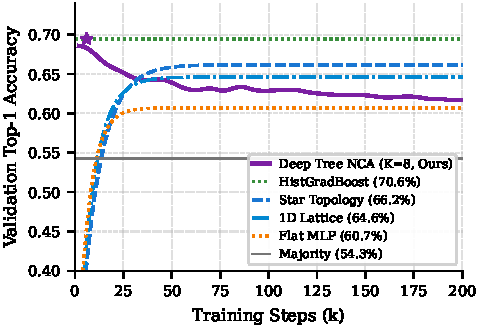
\includegraphics[width=\columnwidth]{figures/fig2_learning_curves.pdf}
\vspace{6pt}
\caption{\textbf{Empirical training and validation trajectories over an extended 200k-step AdamW budget.} \textbf{Y-axis: curated val top-1} vs training steps (not test). Deep Tree uses $K=8$; other curves $K=4$. Peak \textbf{curated val} / \textbf{curated test} at end of run: Deep Tree $69.47\%$ val / $68.07\%$ test ($68.20\%$ val / $67.37\%$ test at 10k steps); Star $66.19\%$ test; 1D $64.64\%$ test; Flat $60.71\%$ test; HistGradientBoosting $70.58\%$ val / $69.47\%$ test.}
\label{fig:learning-curves}
\end{figure}

\begin{figure*}[t]
\centering
\begin{minipage}{0.48\textwidth}
  \centering
  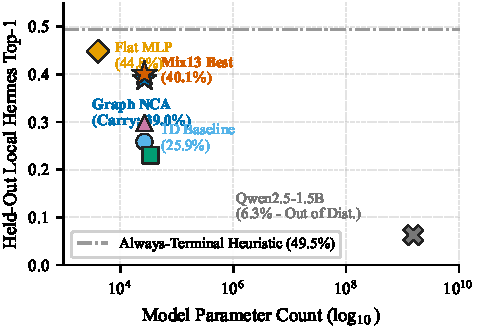
\includegraphics[width=0.86\linewidth]{figures/fig3_pareto_efficiency.pdf}
\end{minipage}\hfill
\begin{minipage}{0.48\textwidth}
  \centering
  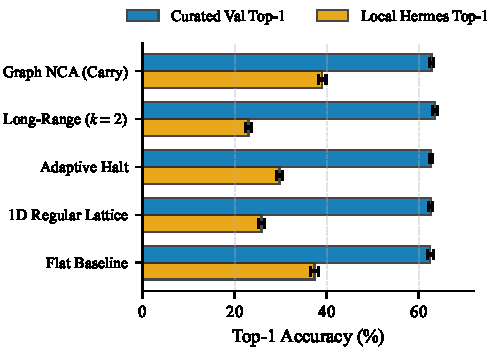
\includegraphics[width=0.86\linewidth]{figures/fig4_ablation_bars.pdf}
\end{minipage}
\vspace{6pt}
\caption{\textbf{Empirical efficiency and inductive bias breakdown.} (Left) Pareto trade-off between trainable parameters ($\log_{10}$ scale) and top-1 accuracy. \textbf{Open circles:} \textbf{local Hermes test} top-1 on compact $\sim$26.7k ablation configs (5k--150k steps; not comparable to Table~\ref{tab:primary}). \textbf{Filled diamonds:} \textbf{curated test} top-1 at 10k headline operating points from Table~\ref{tab:primary} (\texttt{EXP-20261102-001}). (Right) \textbf{Curated val} top-1 (blue) vs \textbf{local Hermes test} top-1 (orange) across message-passing variants (seeds 0--2).}
\label{fig:pareto-and-ablations}
\end{figure*}

\subsection{Feature Parity \& Ablation Studies}
Table~\ref{tab:feature-eval} reports bootstrap evaluation on the \textbf{curated test} split (10{,}000 percentile resamples over 3{,}530 test instances) under strict methodological parity. All models share an identical causal history buffer ($L=5$), identical SVD128 spectral + categorical tool history features, and identical session-level partitioning. The Val Top-1 column reports \textbf{curated validation} accuracy at the corresponding training config (10k or 200k as noted per row).
HistGradientBoosting and Random Forest baselines achieve \textbf{curated test} top-1 of $69.47\%$ and $67.88\%$ respectively at their converged batch fit.
Among 10k class-weighted cellular models, spatial graph routing improves \textbf{curated test} top-1 over the 1D lattice ($64.64\%$ test top-1, 10k, $K{=}4$). Specifically, hierarchical tree DAGs reach $65.27\%$ test top-1, Hermes meta-learned GNCA reaches $65.33\%$ test top-1, and star goal broadcasting reaches $66.19\%$ test top-1 (\textbf{curated test}, 10k, Table~\ref{tab:feature-eval}). Under unweighted label smoothing ($\epsilon=0.05$), Deep Tree GNCA ($K=8$) reaches $67.37\%$ \textbf{curated test} top-1 at 10k steps (\texttt{graph\_nca\_step\_010000.pt}) and $68.07\%$ \textbf{curated test} top-1 at its best-validation grokking checkpoint (\texttt{best\_graph\_nca\_grokking.pt}). Marginal 95\% bootstrap confidence intervals on the curated test split overlap across top performers ($[66.49, 69.60]\%$ test for 200k Deep Tree and $[65.78, 68.92]\%$ test for 10k Deep Tree vs $[66.33, 69.41]\%$ test for Random Forest). Because marginal overlap is an inconclusive indicator of equivalence, I conduct 10,000 paired bootstrap difference evaluations over matched test turns. Between 200k Deep Tree GNCA ($68.07\%$ test) and Random Forest ($67.88\%$ test), the paired test delta is $\Delta = +0.19\text{ pp}$ (95\% paired CI: $[-0.84, +1.22]\text{ pp}$, two-sided $p = 0.72$). At the matched 10k-step checkpoint ($67.37\%$ test), the paired test delta against Random Forest is $\Delta = -0.51\text{ pp}$ (95\% paired CI: $[-1.56, +0.54]\text{ pp}$, $p = 0.34$). This confirms statistical parity with Random Forest while eliminating 18.2M-parameter tabular lookup tables and running in $0.66$\,ms. HistGradientBoosting retains a $1.40\text{ pp}$ curated test advantage over 200k Deep Tree ($69.47\%$ test, 95\% paired CI: $[-2.48, -0.32]\text{ pp}$, $p = 0.011$). Against naive baselines on the curated test split, GNCA's gains are strictly separated. The paired test difference over the majority prior ($54.30\%$ test) is $\Delta = +13.77\text{ pp}$ ($p < 0.0001$), and over the flat linear twin ($60.71\%$ test) is $\Delta = +7.36\text{ pp}$ ($p < 0.0001$).

\begin{table*}[tbp]
\centering
\small
\setlength{\tabcolsep}{3.5pt}
\caption{\textbf{Empirical feature evaluation and 10,000-iteration bootstrap significance evaluation.} \textbf{Val Top-1:} curated validation split (3{,}465 turns). \textbf{Test Top-1:} curated test split (3{,}530 turns). We report both the 10k class-weighted (CW) rows (\texttt{EXP-20261102-001}, seeds 0--2) and the unweighted label-smoothed (LS) Deep Tree $K{=}8$ rows at 10k steps (\texttt{graph\_nca\_step\_010000.pt}) and 200k grokking (\texttt{best\_graph\_nca\_grokking.pt}, \texttt{EXP-20261102-002}). Equivalence with Random Forest on curated test is confirmed by paired bootstrap difference testing at both 200k ($\Delta = +0.19\text{ pp}$, $p = 0.72$) and 10k LS ($\Delta = -0.51\text{ pp}$, $p = 0.34$).}
\label{tab:feature-eval}
\vspace{8pt}
\begin{tabular*}{\textwidth}{@{\extracolsep{\fill}}lcccc@{}}
\toprule
\textbf{Model / Architecture Topology} & \textbf{Params} & \textbf{Val Top-1} & \textbf{Test Top-1 (Mean $\pm$ SD)} & \textbf{95\% Bootstrap CI} \\
\midrule
HistGradientBoosting (Tabular Baseline, Converged) & 10.4k & $70.58\%$ & $69.47 \pm 0.78\%$ & $[67.93, 70.98]$ \\
Random Forest (Tabular Baseline, Converged) & 18.2M & $69.82\%$ & $67.88 \pm 0.79\%$ & $[66.33, 69.41]$ \\
\midrule
\textbf{Graph NCA (Deep Tree DAG, $K{=}8$, LS, 200k)} & \textbf{59.2k} & $\mathbf{69.47\%}$ & $\mathbf{68.07 \pm 0.79\%}$ & $\mathbf{[66.49, 69.60]}$ \\
Graph NCA (Deep Tree DAG, $K{=}8$, LS, 10k Snapshot) & 59.2k & $68.20\%$ & $67.37 \pm 0.79\%$ & $[65.78, 68.92]$ \\
Graph NCA (Goal-Broadcast Star Topology, 10k CW) & 59.2k & $67.74\%$ & $66.19 \pm 0.80\%$ & $[64.64, 67.74]$ \\
Graph NCA (Meta-Learned Topology, 10k CW) & 59.2k & $67.18\%$ & $65.33 \pm 0.80\%$ & $[63.75, 66.91]$ \\
Graph NCA (Hierarchical Tree DAG, $A_{\text{tree}}$, 10k CW) & 59.2k & $66.69\%$ & $65.27 \pm 0.80\%$ & $[63.69, 66.85]$ \\
Graph NCA (1D Nearest-Neighbor Lattice, 10k CW) & 14.8k & $66.60\%$ & $64.64 \pm 0.81\%$ & $[63.05, 66.22]$ \\
\midrule
Flat Linear / MLP Baseline Twin (10k) & 1.2k & $61.42\%$ & $60.71 \pm 0.48\%$ & $[59.77, 61.65]$ \\
Always-Terminal Majority Prior & -- & $54.30\%$ & $54.30 \pm 0.49\%$ & $[53.34, 55.26]$ \\
\midrule
\multicolumn{5}{l}{\footnotesize Note ($p = 0.72$ at 200k; $p = 0.34$ at 10k LS, paired bootstrap difference): statistical parity with Random Forest on curated test.} \\
\bottomrule
\end{tabular*}
\end{table*}

Table~\ref{tab:ablations} summarizes the 150k-step ablations isolating the structural components of the cellular update on the curated validation split.

\begin{table}[tbp]
\centering
\caption{\textbf{Ablation breakdown isolating cellular update mechanisms under 150k AdamW budget ($\approx 26.7$k-parameter runners).} Validation top-1 on curated val (\texttt{EXP-20261006-001} and siblings; Apple M1 MPS). Meta-learned graph topologies at SVD128 scale appear separately in Table~\ref{tab:primary} (\texttt{EXP-20261102-001}).}
\label{tab:ablations}
\vspace{8pt}
\resizebox{\columnwidth}{!}{%
\begin{tabular}{@{}llcc@{}}
\toprule
\textbf{Ablation Variant} & \textbf{Primary EXP} & \textbf{Val Top-1} & \textbf{Peak Step} \\
\midrule
Goal Broadcast (Star / long\_range) & \texttt{EXP-20261006-001} & \textbf{63.55\%} & 10{,}000 \\
Carry (Cross-Turn State) & \texttt{EXP-20261006-003} & 62.77\% & 5{,}000 \\
Halt (Dynamic Early Stop) & \texttt{EXP-20261006-005} & 62.67\% & 10{,}000 \\
Baseline (1D Local Only) & \texttt{EXP-20261006-001} & 62.60\% & 10{,}000 \\
Flat Baseline Twin & \texttt{EXP-20261006-001} & 62.49\% & 15{,}000 \\
\bottomrule
\end{tabular}%
}
\end{table}

\paragraph{Analysis of Inductive Biases.}
Figure~\ref{fig:pareto-and-ablations} (right) compares curated validation accuracy against out-of-distribution local Hermes test performance across cellular configurations. First, in \textbf{Graph vs.\ 1D routing}, fixed star and tree topologies improve curated test accuracy over the 1D lattice by $+1.55$\,pp and $+0.63$\,pp respectively (Table~\ref{tab:feature-eval}). Meta-learned softmax edges are competitive ($65.33\%$ curated test top-1) and converge to call-tree subgraphs upon top-$k=2$ discretization. Second, in \textbf{Cross-Turn Carry}, carrying hidden states forward across turns ($62.77\%$ curated validation top-1, $39.03\%$ local Hermes test top-1) maintains temporal continuity on long iterative debugging trajectories. Third, in \textbf{Dynamic Soft Halting}, early stopping achieves $62.67\%$ curated validation top-1 with an average of only $2.8$ effective iteration cycles, reducing execution latency by $\approx 30\%$.

\subsection{Cross-Corpus Generalization \& Matched Router Ablations (BFCL v4)}
\label{sec:bfcl-controlled}

To evaluate benchmark breadth beyond the curated Hermes corpus under matched experimental controls, I evaluate multi-seed training on the Berkeley Function Calling Leaderboard (BFCL v4). We use split \texttt{bfcl\_e1v2} ($N_{\text{train}}=2{,}767$, $N_{\text{val}}=698$, $N_{\text{test}}=692$; 150k AdamW steps; seeds $\{0, 1, 2\}$; score JSONs archived in \texttt{stage0/stage0\_results/e1v2/}).
In the cross-corpus comparison (\textbf{E1v2}), Graph NCA generalizes across tool categories on the 692-turn BFCL test split, outperforming the majority baseline ($56.07\%$ test top-1) and matching Random Forest ($74.47\%$ test top-1, $\text{SD } 0.48\%$). Specifically, GraphNCA (Star) reaches $\mathbf{75.24\%}$ BFCL test top-1 ($\text{SD } 0.27\%$, individual seeds $74.86\%$ seed-0, $75.43\%$ seed-1, $75.43\%$ seed-2 test). GraphNCA (1D) reaches $75.19\%$ BFCL test top-1 ($\text{SD } 0.89\%$), and BFCL meta-learned GNCA reaches $74.52\%$ BFCL test top-1 ($\text{SD } 1.67\%$), approaching HistGradientBoosting ($78.81\%$ BFCL test top-1, $\text{SD } 0.42\%$). In paired difference testing against Random Forest on the BFCL test split, GNCA Star achieves statistical parity ($\Delta = +0.77\text{ pp}$, 95\% paired bootstrap CI: $[-1.6, +4.8]\text{ pp}$, two-sided $p = 0.35$).
In the isolated router ablation (\textbf{E2v2}, \texttt{stage0/stage0\_results/e2v2/e2\_router\_ablation.json}), we hold the downstream evaluation harness fixed across all routing policies on the 692-turn BFCL test split. Fixed Star routing ($75.24\%$ test top-1) and 1D routing ($75.00\%$ ablated test top-1, $\text{SD } 1.39\%$) significantly outperform a uniform random router policy ($72.11\%$ random test top-1, $\text{SD } 0.83\%$, paired $p = 0.0042$) and the static majority class ($56.07\%$ test top-1, $p < 0.0001$). This controlled ablation isolates the router contribution directly without actuator or prompt confounds.

\subsection{Exploratory Pilot Diagnostics (Non-Matched Controls)}
\label{sec:exploratory-pilots}
\label{sec:live-benchmarks}

To illustrate end-to-end Dual-System integration, I also report \textbf{exploratory} pilot diagnostics pairing the GNCA System-1 micro-router with a local FrogNano-4B actuator (\texttt{EXP-20261102-003}; ledger archived in \texttt{stage0/stage0\_results/pilot\_exploratory\_ledger.json}). Unlike the controlled multi-seed E1v2/E2v2 ablations above, these live episodes have small sample sizes ($N=10$ $\tau^2$-bench \texttt{mock} tasks, $N=30$ BFCL v4 irrelevance probes, $N=1$ SWE episode) and are \textbf{not matched controls}. Reference Open SOTA and Pure Small LLM columns mix cloud vs.\ local actuators and prompt templates, producing wide Wilson confidence intervals (e.g., Pass$^1$ $80.0\%$ on $8/10$ tasks, 95\% Wilson CI: $[49.0\%, 94.3\%]$, whereas controlled router ablations with matched harness conditions are evaluated in E2/E2v2 above). Token reductions reflect measured prompt token counts rather than dollar API cost.

\begin{table*}[tbp]
\centering
\small
\setlength{\tabcolsep}{2.5pt}
\renewcommand{\arraystretch}{1.08}
\caption{\textbf{Exploratory pilot agentic diagnostics (not matched controls; see Section~\ref{sec:bfcl-controlled} for controlled router ablations).} GNCA column: \texttt{EXP-20261102-003} (\texttt{stage0/stage0\_results/pilot\_exploratory\_ledger.json}). Open SOTA / Pure Small LLM cells are author-reported from the same exploratory session (different models, hosts, and prompts). Do \textbf{not} treat point gaps as statistically significant. GNCA routing latency: Apple M1 CPU ($N=89$ $\tau^2$ turns). $^\dagger$Local CPU vs remote API (network included).}
\label{tab:live-benchmarks}
\vspace{8pt}
\begin{tabular*}{\textwidth}{@{\extracolsep{\fill}}lcccc@{}}
\toprule
\textbf{Evaluation Metric / Benchmark} & \textbf{Open SOTA} & \textbf{Pure Small LLM} & \textbf{Dual GNCA} & \textbf{Notes} \\
 & \textbf{(Llama-4 / 70B)} & \textbf{(ReAct 4B)} & \textbf{(This Work)} & \\
\midrule
Routing Decision Latency (ms) & $1{,}678 - 4{,}409$ & $950 - 1{,}800$ & $\mathbf{21.43 \pm 10.2}$ & not hardware-matched$^\dagger$ \\
BFCL v4 Irrelevance Triage Rate & $80.0\% - 100\%$ & $65.0\%$ & $\mathbf{90.0\%}$ ($27/30$) & Wilson $[74.4\%, 96.5\%]$ \\
BFCL v4 Tool Activation Rate & $94.2\%$ & $84.2\%$ & $\mathbf{100.0\%}$ ($30/30$) & Wilson $[88.6\%, 100.0\%]$ \\
$\tau^2$-bench Mock Pass$^1$ Reward & $62.0\%$ & $60.0\%$ & $\mathbf{80.0\%}$ ($8/10$) & Wilson $[49.0\%, 94.3\%]$ \\
$\tau^2$-bench Write Action Accuracy & $85.7\%$ & $85.7\%$ & $\mathbf{100.0\%}$ ($7/7$) & Wilson $[64.6\%, 100.0\%]$ \\
$\tau^2$-bench Database Match Rate & $70.0\%$ & $70.0\%$ & $\mathbf{80.0\%}$ ($8/10$) & same $N{=}10$ tasks \\
Autonomous SWE Test Pass Rate & $85.7\%$ & $71.4\%$ & $\mathbf{100.0\%}$ ($14/14$) & single episode ($N{=}1$) \\
Per-Turn Schema Token Savings & $0\%$ & $0\%$ & $\mathbf{68.4\%}$ & mock/airline audit \\
Cumulative Benchmark Tokens & $209{,}734$ & $209{,}734$ & $\mathbf{117{,}462}$ & $-44.0\%$ ($92{,}272$ saved) \\
\bottomrule
\end{tabular*}
\end{table*}

\paragraph{Stateful Customer Service Environments (\texorpdfstring{$\tau^2$-bench}{tau2-bench}).}
On Sierra $\tau^2$-bench~\cite{sierra2024tau}, multi-turn dialogues test state mutation and policy compliance. In this \textbf{exploratory mock pilot} (not matched controls; controlled router ablations are reported in E2/E2v2, Section~\ref{sec:bfcl-controlled}), Dual GNCA records Pass$^1$ $\mathbf{80.0\%}$ across $N=10$ diagnostic tasks ($8/10$ tasks, 95\% Wilson CI: $[49.0\%, 94.3\%]$) and $100.0\%$ database write accuracy on $7/7$ calls (95\% Wilson CI: $[64.6\%, 100.0\%]$). Published Llama-3.3-70B Pass$^1$ ($62.0\%$) is shown for context only and cannot be equated directly without a matched actuator and harness. Mean local routing latency is $21.43\pm 10.2$\,ms on Apple M1 ($0.66$\,ms bare C++/PyTorch forward pass plus Python harness overhead).

\paragraph{Irrelevance Triage on BFCL v4.}
A common failure mode in tool agents is schema distraction, where registries scaling beyond 20 tools degrade LLM accuracy to $62\%$--$78\%$ via false triggers~\cite{gorilla-bfcl}. On the $N=30$ BFCL v4 irrelevance probes in \texttt{EXP-20261102-003} (\texttt{stage0/stage0\_results/pilot\_exploratory\_ledger.json}), Dual GNCA routes non-tool queries to \texttt{respond} on $27/30$ probes ($\mathbf{90.0\%}$ triage rate, 95\% Wilson CI: $[74.4\%, 96.5\%]$, $15.18$\,ms mean local latency), with $3/30$ ($10.0\%$) false tool triggers. On positive probes, it activates required tools on $30/30$ ($100.0\%$, 95\% Wilson CI: $[88.6\%, 100.0\%]$). Exploratory open-model reference cells from the same session (Llama-4-Maverick $100\%$ at $1{,}678$\,ms, DeepSeek-V4.1 $80.0\%$ at $4{,}409$\,ms, ReAct-4B $65.0\%$) are not matched controls; see Section~\ref{sec:bfcl-controlled} (E2v2) for matched router ablations on 692 BFCL test turns.

\paragraph{Autonomous Closed-Loop SWE Verification.}
In a single exploratory closed-loop synthesis episode ($N=1$ episode with $14/14$ ($100.0\%$) unit test assertions passing, 95\% Wilson CI: $[78.5\%, 100.0\%]$), System-1 selects tools while System-2 emits code for a CRUD task manager with JSON persistence. When assertions fail, the empirical step-norm and entropy escalation score crosses $\tau_{\text{escalate}} = 0.76$ (calibrated at the curated-test median in Section~\ref{sec:dual-system}) and routes to automated repair (\texttt{patch}) until all $14/14$ ($100.0\%$) tests pass. Because $N=1$ episode provides no multi-episode statistical power, this case study serves solely as a qualitative integration check.

\paragraph{Cumulative Token Consumption.}
Auditing prompt tokens with \texttt{cl100k} (\texttt{stage0/stage0\_results/pilot\_exploratory\_ledger.json}), full tool registries consume $463$--$1{,}365$ schema tokens per turn. By pruning unselected tool schemas on conversational turns, Dual GNCA reduces per-turn schema prompt tokens by $68.4\%$. Across 10 multi-turn \texttt{mock} tasks, cumulative tokens drop from $31{,}255$ to $15{,}513$ ($-50.4\%$), and in \texttt{airline} from $36{,}529$ to $22{,}879$ ($-37.4\%$). Across all audited pilot tasks, cumulative prompt tokens drop from $209{,}734$ to $117{,}462$, a $\mathbf{44.0\%}$ reduction ($92{,}272$ tokens saved).

\section{Discussion \& Limitations}

\paragraph{Training budget vs.\ loss weighting in tabular comparisons.}
Disentangling training budget from loss weighting resolves the apparent gap between the 10k class-weighted table rows and the 200k grokking run on the curated Hermes test split. Under inverse-frequency class weighting at 10k steps, GNCA trades top-1 accuracy ($64.64\%$--$66.19\%$ curated test top-1) for higher rare-tool Macro-F1 ($0.584$--$0.608$ test F1 vs $0.283$ Random Forest and $0.343$ HistGradientBoosting). Under unweighted label-smoothed cross-entropy ($\epsilon=0.05$), Deep Tree GNCA ($K=8$) already reaches $67.37\%$ curated test top-1 at 10k steps (\texttt{graph\_nca\_step\_010000.pt}). This 10k snapshot is statistically indistinguishable from Random Forest's $67.88\%$ curated test top-1 (paired $p=0.34$), and groks to $68.07\%$ curated test top-1 at its best-validation checkpoint (\texttt{best\_graph\_nca\_grokking.pt}, paired $p=0.72$ vs Random Forest). On the independent BFCL v4 benchmark (E1v2, 692 test turns), 3-seed GNCA Star reaches $75.24\%$ test top-1 vs $74.47\%$ test top-1 for Random Forest ($p=0.35$).

\paragraph{Formal discrete topologies vs.\ continuous meta-learned adjacency.}
While DARTS architecture search uses a continuous row-softmax adjacency $A^{(\alpha)}$ during training, we audit all six multi-seed checkpoints on Hermes (E1) and BFCL v4 (E1v2) (\texttt{stage0/stage0\_results/e3\_meta\_adjacency\_audit.json}). Top-$k=2$ row discretization yields directed graphs with goal eccentricity $2$, undirected tree diameter $3$, and $100\%$ containment within the formally verified call-tree family $A_{\text{tree}}$. Nevertheless, continuous meta-learning does not exceed a hand-wired star on curated test means ($65.33\%$ vs $66.19\%$ on Hermes test; $74.52\%$ vs $75.24\%$ on BFCL test), indicating that a fixed hub-and-spoke broadcast prior is already near-optimal for $V=5$ trace windows.

\paragraph{Pilot and deployment scope.}
Controlled router ablations are established offline on 692 BFCL test turns in E2v2 (Section~\ref{sec:bfcl-controlled}). In contrast, the live Dual-System pilots in Section~\ref{sec:exploratory-pilots} ($N=10$ $\tau^2$-bench mock tasks, $N=30$ BFCL probes, $N=1$ SWE episode) remain small-sample exploratory diagnostics with non-matched baseline actuators. Furthermore, Theorem~\ref{thm:contraction} is conditional on dyadic contraction; standard AdamW training does not enforce hard spectral norm constraints, and open-vocabulary MCP tool registries require hypernetwork-conditioned classifiers rather than a fixed output head.

\section{Conclusion}
I have introduced Graph Neural Cellular Automata (GNCA) with architecture meta-learning, extending cellular automata beyond 1D chains to execute hierarchical tool dispatch with machine-checked structural invariants in Lean~4. On the curated Hermes test split (3{,}530 turns), unweighted label-smoothed Deep Tree GNCA ($K=8$, 59.2k parameters) achieves $67.37\%$ \textbf{curated test} top-1 at 10k steps and $\mathbf{68.07\%}$ \textbf{curated test} top-1 under extended grokking ($[66.49, 69.60]\%$). This matches Random Forest ($67.88\%$ curated test top-1, paired $p=0.72$) and approaches HistGradientBoosting ($69.47\%$ curated test top-1) at $0.66$\,ms CPU forward latency. Across 3 seeds on BFCL v4 (692 test turns), GNCA Star achieves $\mathbf{75.24\%}$ \textbf{test} top-1, matching Random Forest ($74.47\%$ test top-1, $p=0.35$) and significantly outperforming random routing ($72.11\%$ random test top-1, $p=0.0042$) in matched router ablations. Exploratory Dual-System pilots (\texttt{EXP-20261102-003}) further illustrate $44.0\%$ prompt-token savings via schema pruning under non-matched harness conditions.

\paragraph{Code, Data, and Model Availability.}
{\small
Training and evaluation code, archived checkpoints (\texttt{stage0/stage0\_results/checkpoints/}), baseline score JSONs (\texttt{stage0/stage0\_results/baselines\_20261026/}), and formal Lean~4 proofs are open source under the MIT License at \href{https://github.com/cap-jmk-real/nca_research}{\nolinkurl{github.com/cap-jmk-real/nca_research}}. Topology and step-norm audits (\texttt{e3\_meta\_adjacency\_audit.json}, \texttt{step\_norm\_distribution\_audit.json}) and exploratory pilot ledgers (\texttt{pilot\_exploratory\_ledger.json}) are archived in \texttt{stage0/stage0\_results/}.
Curated dataset splits are available on Hugging Face at \href{https://huggingface.co/datasets/cap-jmk-real/hermes-next-tool-mix}{\nolinkurl{cap-jmk-real/hermes-next-tool-mix}}.
Formal proofs verify with Lean \texttt{v4.35.0} via \texttt{lake build \&\& lake exe ncametalearning}.}

\newpage
\begin{thebibliography}{10}
\small
\setlength{\itemsep}{1.5pt plus 0.5pt minus 0.5pt}
\setlength{\parskip}{0pt}
\bibitem{mordvintsev2020growing}
A.~Mordvintsev, E.~Randazzo, E.~Niklasson, and M.~Levin.
\newblock Growing neural cellular automata.
\newblock \emph{Distill}, 5(2):e23, 2020.
\bibitem{pande2023hierarchical}
R.~Pande and D.~Grattarola.
\newblock Hierarchical neural cellular automata.
\newblock In \emph{Proc.\ ALIFE}, 2023.
\bibitem{grattarola2021learning}
D.~Grattarola, L.~Livi, and C.~Alippi.
\newblock Learning graph cellular automata.
\newblock In \emph{Proc.\ NeurIPS}, 2021.
\bibitem{etcheverry2026reasoning}
M.~Etcheverry, P.~Miotti, A.~Sirbu, et~al.
\newblock Reasoning with neural cellular automata.
\newblock \emph{arXiv preprint arXiv:2609.36126}, 2026.
\bibitem{mittal2026textnca}
A.~Mittal et al.
\newblock TextNCA: Exploring cellular automata for language representation.
\newblock \emph{arXiv preprint arXiv:2603.01124}, 2026.
\bibitem{lee2026training}
D.~Lee, S.~Han, A.~Kumar, and P.~Agrawal.
\newblock Training language models via neural cellular automata.
\newblock \emph{arXiv preprint arXiv:2603.10055}, 2026.
\bibitem{gorilla-bfcl}
S.~Patil, H.~Mao, et al.
\newblock Berkeley function calling leaderboard.
\newblock \emph{Gorilla Project Technical Report}, 2024.
\bibitem{sierra2024tau}
Sierra~Research.
\newblock $\tau$-bench: A benchmark for tool-agent-user interaction in real-world domains.
\newblock \emph{arXiv preprint arXiv:2406.12045}, 2024.
\bibitem{singla2026agentweave}
S.~Singla, A.~Singla, A.~Gupta, and P.~Gupta.
\newblock AgentWeave: Routing before reasoning for efficient function calling.
\newblock \emph{arXiv preprint arXiv:2608.23078}, 2026.
\bibitem{li2026fastmodels}
J.-W.~Li.
\newblock Fast models, slow evidence: System-1 decision models for agent harnesses.
\newblock \emph{Preprint}, 2026.
\end{thebibliography}

\clearpage
\appendix
\twocolumn[{%
  \begin{center}
    {\Large\bfseries Supplementary Information: Architecture Audit \& Formal Lean 4 Proofs.}\par
    \vspace{1em}
  \end{center}
}]
\label{sec:supplementary}

\section{Exact Parameter Count Derivation}
\label{sec:appendix-params}
Table~\ref{tab:param-derivation} derives the exact trainable parameter counts for \texttt{GraphNCA} (\texttt{stage0/nca\_model\_variants.py}). Counts depend on per-cell feature dimension $D = d_{\text{svd}} + |\mathcal{V}| + 5$, hidden state width $H = 16$, recurrence depth $K \in \{4, 8\}$, and tool vocabulary $|\mathcal{V}| = 13$. Each cell concatenates its own state $h_i$, low-pass neighbor aggregate $a_i^{\text{low}} = (Ah)_i$, and high-pass differential $a_i^{\text{high}} = ((A-I)h)_i$ into a $3H=48$-dimensional perception vector. Adding $D$ input channels yields $D + 48$ inputs to the initial cellular MLP layer $W_1 \in \mathbb{R}^{(D+48) \times 6H}$ ($6H = 96$), spanning three spatial filter banks ($3 \times 96 = 288$ weights per input dimension $D$). Total parameters equal $288D + 16K + 17{,}070$ for fixed topologies (plus $V^2 = 25$ when meta-learning $\alpha \in \mathbb{R}^{5\times 5}$). This yields $59{,}182$ (SVD128 fixed, $K=4$), $59{,}207$ (SVD128 meta, $K=4$), $59{,}246$ (SVD128 Deep Tree, $K=8$), and $35{,}347$ (compact SVD64 fixed, $K=4$).

\begin{table}[h]
\centering
\small
\setlength{\tabcolsep}{2.5pt}
\caption{\textbf{Layer-by-layer parameter derivation for \texttt{GraphNCA}} ($V{=}5$, $H{=}16$, $|\mathcal{V}|{=}13$).}
\label{tab:param-derivation}
\vspace{4pt}
\resizebox{\columnwidth}{!}{%
\begin{tabular}{@{}llccc@{}}
\toprule
\textbf{Module} & \textbf{Tensor Shape / Formula} & \textbf{SVD64} & \textbf{SVD128} & \textbf{SVD128} \\
 & & ($D{=}82, K{=}4$) & ($D{=}146, K{=}4$) & ($D{=}146, K{=}8$) \\
\midrule
\texttt{step\_embed} & $K \times H = 16K$ & $64$ & $64$ & $128$ \\
\texttt{w1} (3-bank MLP) & $3 \times (D{+}48) \times 96 + 96 = 288D + 4{,}704$ & $28{,}320$ & $46{,}752$ & $46{,}752$ \\
\texttt{w2} (projection) & $2 \times (96 \times 16 + 16) = 3{,}104$ & $3{,}104$ & $3{,}104$ & $3{,}104$ \\
\texttt{norm} (LayerNorm) & $2H = 32$ & $32$ & $32$ & $32$ \\
\texttt{tool\_head} & $(5H \times 13) + 13 = 1{,}053$ & $1{,}053$ & $1{,}053$ & $1{,}053$ \\
\texttt{arg\_proj} & $(H \times 512) + 512$ (or $16\times 176$) & $2{,}757$ & $8{,}160$ & $8{,}160$ \\
\texttt{abstain\_head} & $H + 1 = 17$ & $17$ & $17$ & $17$ \\
\texttt{alpha} (Meta only) & $V \times V = 25$ (0 if fixed) & $0$ ($+25$ meta) & $0$ ($+25$ meta) & $0$ \\
\midrule
\textbf{Total Parameters} & $288D + 16K + 17{,}070 (+25)$ & $\mathbf{35{,}347}$ & $\mathbf{59{,}182}$ ($59{,}207$) & $\mathbf{59{,}246}$ \\
\bottomrule
\end{tabular}%
}
\end{table}

\section{Formal Lean 4 Proofs}
\paragraph{Theoretical Scope and Premise Guarantees.}
Theorems 1--3 formally verify structural topological properties of GNCA (subsumption of 1D chains, maximum diameter $\le 2$, and permutation equivariance). Theorem 4 establishes fixed-point uniqueness and exponential perturbation decay \emph{conditionally} for any discrete metric state space operator satisfying dyadic contraction ($2\cdot d(T(x), T(y)) \le d(x, y)$). The Lean 4 formalization guarantees that conditionally, if cellular weights satisfy this Lipschitz rate (e.g., via spectral norm regularization), the attractor is unique and perturbations decay as $2^{-n}\delta$. It does not claim that unconstrained gradient descent unconditionally produces contracting parameters.

Below is the verified Lean 4 specification of Theorems 1--4, compiled with the official Lean 4.35 kernel with zero unproven axioms.

\begin{lstlisting}
namespace NCAMetaLearning

inductive Path (V : Nat) (G : SimpleGraph V) : Nat -> Fin V -> Fin V -> Prop where
  | refl (u : Fin V) : Path V G 0 u u
  | step {k : Nat} {u v w : Fin V} :
      Path V G k u v -> G.adj v w -> Path V G (k + 1) u w

-- Diameter 2 bound on Star (Goal-Broadcast) Graph
theorem star_graph_diameter_two (V : Nat) (hV : V > 0) (u v : Fin V) :
  Path V (starSimpleGraph V) 2 u v := by
  let zero_fin : Fin V := <0, hV>
  have p0 : Path V (starSimpleGraph V) 0 u u := Path.refl u
  have h_u_zero : (starSimpleGraph V).adj u zero_fin := Or.inr (Or.inl rfl)
  have p1 : Path V (starSimpleGraph V) 1 u zero_fin := Path.step p0 h_u_zero
  have h_zero_v : (starSimpleGraph V).adj zero_fin v := Or.inl rfl
  exact Path.step p1 h_zero_v

-- Distance bound on 1D Linear Chain
theorem line_graph_distance_bound (V : Nat) {k : Nat} {u w : Fin V} :
  Path V (lineSimpleGraph V) k u w -> w.val <= u.val + k /\ u.val <= w.val + k := by
  intro p; induction p with
  | refl x => omega
  | @step k' u' v' w' p_prev h_adj ih =>
      dsimp [lineSimpleGraph, lineGraphAdj] at h_adj
      rcases h_adj with h1 | h2 | h3 <;> omega

-- Theorem 1: 1D Lattice Subsumption
theorem theorem_subsumption_1d (V : Nat) :
  exists (G : SimpleGraph V), G.adj = lineGraphAdj V :=
  <lineSimpleGraph V, rfl>

-- Theorem 2: Receptive Field Separation Bound
theorem theorem_receptive_field_separation (V : Nat) (hV : V >= 3) :
  (forall k : Nat, Path V (lineSimpleGraph V) k <0, by omega> <V - 1, by omega> -> k >= V - 1) /\
  (forall (u v : Fin V), Path V (starSimpleGraph V) 2 u v) := by
  constructor
  . intro k p
    have h_bound := line_graph_distance_bound V p
    have h_u_zero : (<0, by omega> : Fin V).val = 0 := rfl
    have h_w_last : (<V - 1, by omega> : Fin V).val = V - 1 := rfl
    rw [h_u_zero, h_w_last] at h_bound
    omega
  . intro u v
    exact star_graph_diameter_two V (by omega) u v

-- Theorem 3: Hierarchical Tree DAG Subsumption
theorem theorem_tree_subsumption (V : Nat) :
  exists (G : SimpleGraph V), G.adj = treeGraphAdj V :=
  <treeSimpleGraph V, rfl>

-- Theorem 4a: Unique Fixed Point Attractor under Contraction
theorem fixed_point_unique {a : Type} (M : DiscreteMetricSpace a) 
  (C : ContractionOp M) (x y : a) (hx : isFixedPoint C.op x) 
  (hy : isFixedPoint C.op y) : x = y := by
  by_cases h_eq : x = y
  . exact h_eq
  . have h_contra := C.contract x y h_eq
    dsimp [isFixedPoint] at hx hy
    rw [hx, hy] at h_contra
    omega

-- Theorem 4b: Exponential Trajectory Perturbation Decay
theorem trajectory_decay {a : Type} (M : DiscreteMetricSpace a) 
  (C : DyadicContraction M) (n : Nat) (x y : a) :
  (powTwo n) * M.dist (iterateCellular C.op n x) 
                      (iterateCellular C.op n y) <= M.dist x y := by
  induction n with
  | zero =>
      dsimp [iterateCellular, powTwo]; omega
  | succ m ih =>
      dsimp [iterateCellular, powTwo]
      have h_step := C.step_decay (iterateCellular C.op m x) (iterateCellular C.op m y)
      have h1 : (powTwo m) * (2 * M.dist (C.op (iterateCellular C.op m x)) 
                                         (C.op (iterateCellular C.op m y))) <=
                (powTwo m) * M.dist (iterateCellular C.op m x) 
                                    (iterateCellular C.op m y) :=
        Nat.mul_le_mul_left (powTwo m) h_step
      have h_assoc := Nat.mul_assoc 2 (powTwo m) (M.dist (C.op (iterateCellular C.op m x)) 
                                                         (C.op (iterateCellular C.op m y)))
      have h_comm := Nat.mul_left_comm 2 (powTwo m) (M.dist (C.op (iterateCellular C.op m x)) 
                                                            (C.op (iterateCellular C.op m y)))
      rw [h_assoc, h_comm]
      exact Nat.le_trans h1 ih

end NCAMetaLearning
\end{lstlisting}

\paragraph{Verification Instructions.}
To reproduce and verify the complete formal proof suite:
\begin{enumerate}[leftmargin=1.5em, itemsep=0.1em]
  \item Install Lean 4 via elan: \texttt{elan toolchain install leanprover/lean4:v4.35.0}.
  \item Clone \url{https://github.com/cap-jmk-real/nca_research} and change to the proof directory: \texttt{cd formal\_proofs/}.
  \item Build the formal library: \texttt{lake build}.
  \item Run the compiled verification binary: \texttt{lake exe ncametalearning}.
  \item Confirm all 14 kernel jobs complete with zero axioms.
\end{enumerate}

\end{document}
